\section{角度制御}

\subsection{実験内容}
\subsubsection{P制御}
\subsubsection{パラメータ設定}

4章で述べたように,P コントローラ
\begin{align}
    v_x(t) &= k_{Px} e_x(t),\quad e_x(t) = \theta_x^{\mathrm{ref}}(t) - \theta_x(t) \notag \\
    v_y(t) &= k_{Py} e_y(t),\quad e_y(t) = \theta_y^{\mathrm{ref}}(t) - \theta_y(t)
    \tag{5.1}
\end{align}
を用いると,$\theta_x^{\mathrm{ref}}(s)$ から $\theta_x(s)$ への伝達関数は 2 次遅れ要素
\begin{align}
    \begin{cases}
        T_x(s) = \dfrac{\omega_{nx}^2}{s^2 + 2\zeta_x \omega_{nx} s + \omega_{nx}^2} \\
        T_y(s) = \dfrac{\omega_{ny}^2}{s^2 + 2\zeta_y \omega_{ny} s + \omega_{ny}^2}
    \end{cases}
    \tag{5.2}
\end{align}
となる.ただし,
\begin{tcolorbox}[colframe=black!75!white, colback=white!95!white, boxrule=0.5pt]
\textbf{固有角周波数:} 
$\omega_{nx} = \sqrt{b_x k_{Px}},\quad \omega_{ny} = \sqrt{b_y k_{Py}}$ \\
\textbf{減衰係数:} 
$\zeta_x = \dfrac{a_x}{2\omega_{nx}} = \dfrac{a_x}{2\sqrt{b_x k_{Px}}},\quad
\zeta_y = \dfrac{a_y}{2\omega_{ny}} = \dfrac{a_y}{2\sqrt{b_y k_{Py}}}$
\end{tcolorbox}
である.したがって,P コントローラで指定できるのは,固有角周波数 $\omega_{nx}$,$\omega_{ny}$ か減衰係数 $\zeta_x$,$\zeta_y$ のいずれかである.

たとえば,固有角周波数 $\omega_{nx}$,$\omega_{ny}$ を指定した値 $\omega_{Mx}$,$\omega_{My}$ とするとには,比例ゲイン $k_{Px}$,$k_{Py}$ を
\begin{align}
    \begin{cases}
        k_{Px} = \dfrac{\omega_{Mx}^2}{b_x} \\
        k_{Py} = \dfrac{\omega_{My}^2}{b_y}
    \end{cases}
    \tag{5.4}
\end{align}
とすればよいが,$\omega_{Mx}, \omega_{My}$ を大きくするにつれて比例ゲイン $k_{Px}$,$k_{Py}$ が大きくなり,減衰係数 $\zeta_x$, $\zeta_y$ を零に近づけてしまうため,振動的な応答となってしまう.

また,減衰係数 $\zeta_x$, $\zeta_y$ を指定した値(たとえば $\zeta_{Mx}, \zeta_{My}$)とするとには,比例ゲイン $k_{Px}$,$k_{Py}$ を
\begin{align}
    \begin{cases}
        k_{Px} = \dfrac{a_x^2}{4\zeta_{Mx}^2 b_x} \\
        k_{Py} = \dfrac{a_y^2}{4\zeta_{My}^2 b_y}
    \end{cases}
    \tag{5.5}
\end{align}
とすればよいが,固有角周波数 $\omega_{nx}, \omega_{ny}$ が決まってしまい,速応性を考慮することはできない.

\subsubsection{シミュレーションと実験}

\fbox{\strut \textbf{ステップ 1}}:
MATLAB/Simulink を起動し,カレントディレクトリを \texttt{\textyen Pcont} に移動する.つぎに,4.3 節で定めたパラメータを保存した MAT ファイル ``\texttt{armpara.mat}'',(5.4) 式にしたがって P コントローラを設計する M ファイル ``\texttt{armP.m}'',シミュレーションモデル ``\texttt{sim\_P.slx}''(図\ref{fig:simulink_model_4link2joint}),実機実験モデル ``\texttt{ex\_P.slx}''(図\ref{fig:sim_param})を作成し,\texttt{C:\textbackslash robot\textbackslash Pcont} に保存する.ただし,目標値は
\begin{align}
    \mathrm{Step}\left(\theta_x^{\mathrm{ref}}(t)\right)\colon
    \begin{cases}
        \text{ステップ時間:}0 \\
        \text{初期値:}0 \\
        \text{最終値:}0.3 \\
        \text{サンプル時間:}0
    \end{cases}
    ,\quad
    \mathrm{Step1}\left(\theta_y^{\mathrm{ref}}(t)\right)\colon
    \begin{cases}
        \text{ステップ時間:}0 \\
        \text{初期値:}0 \\
        \text{最終値:}0 \\
        \text{サンプル時間:}0
    \end{cases}
    \tag{5.6}
\end{align}
と設定する.

\begin{figure}[htbp]
    \centering
    \begin{subfigure}[b]{0.7\linewidth}
        \centering
        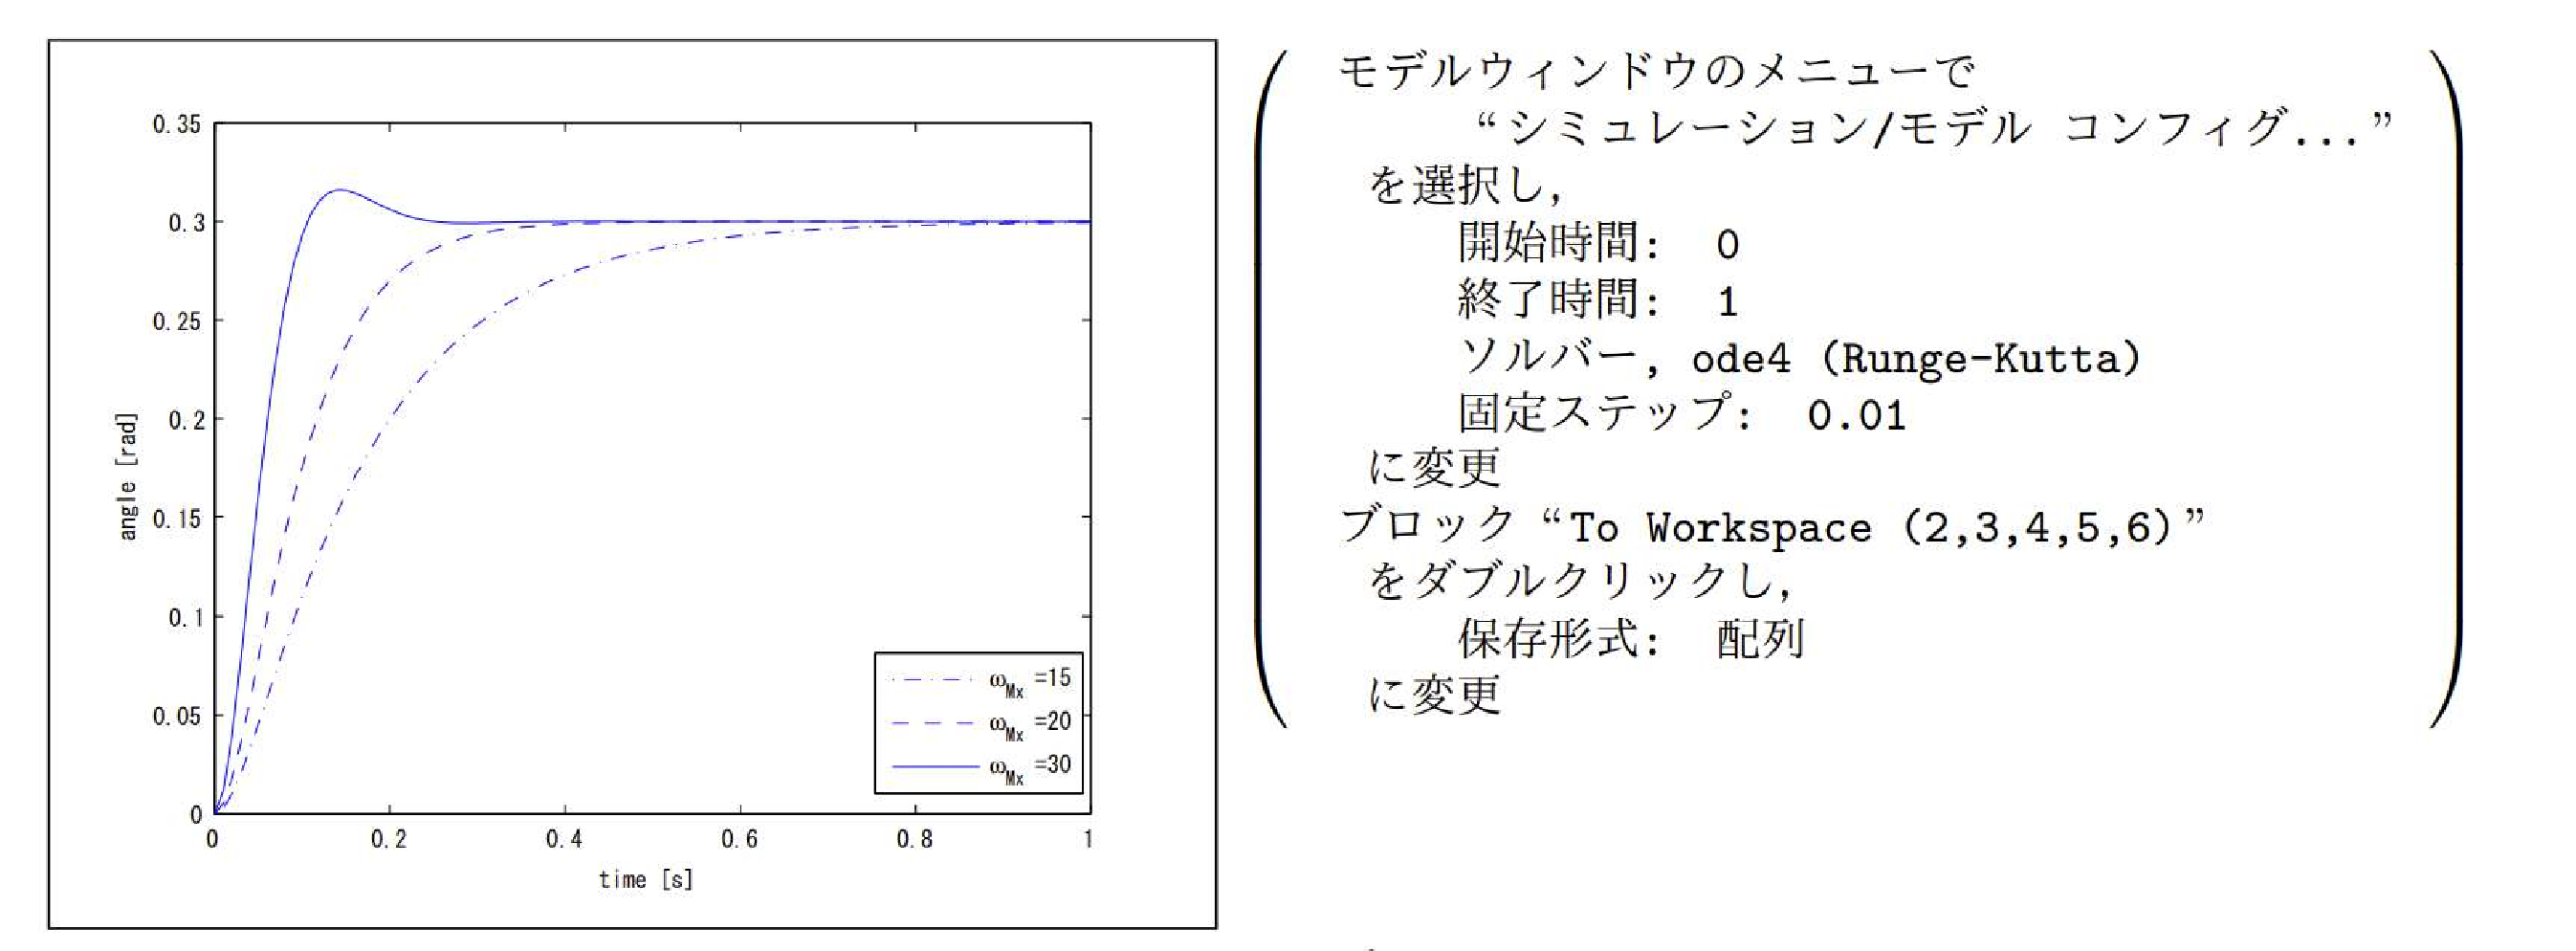
\includegraphics[width=\linewidth]{figure/sim_result_omega.pdf}
        \caption{シミュレーションモデル ``sim\_P.slx''}
    \end{subfigure}
    \hfill
    \begin{subfigure}[b]{0.45\linewidth}
        \centering
        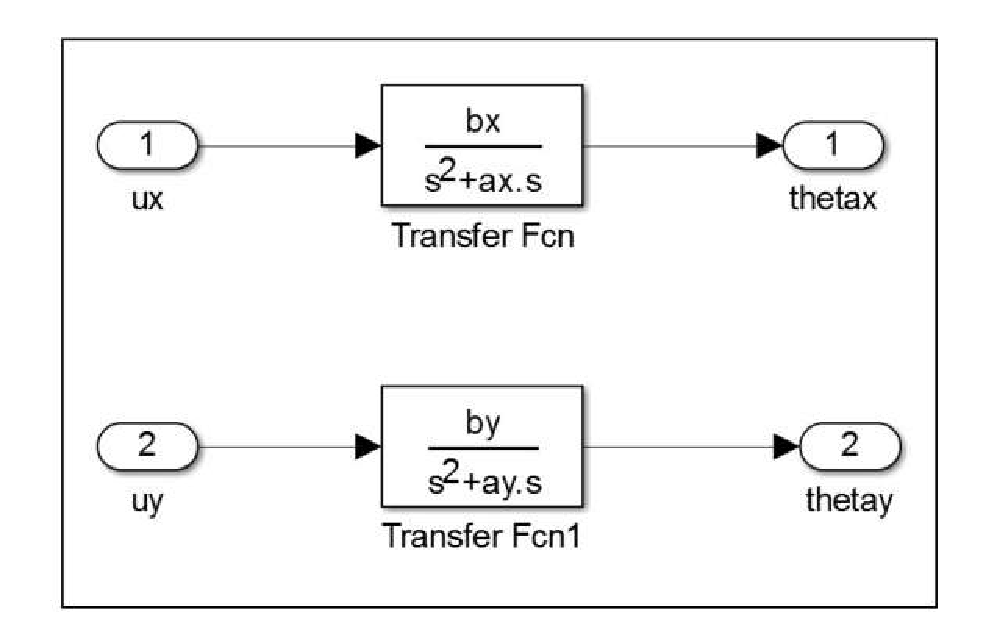
\includegraphics[width=\linewidth]{figure/sim_model_block.pdf}
        \caption{Subsystem ``2D Robot Model'' の内容}
    \end{subfigure}
    \caption{P 制御の Simulink モデル}
    \label{fig:sim_param}
\end{figure}

\noindent
モデルウィンドウのメニューで ``シミュレーション/モデル コンフィグ...'' を選択し,
\begin{itemize}
  \item 開始時間:0
  \item 終了時間:1
  \item ソルバー:ode4 (Runge-Kutta)
  \item 固定ステップ:0.01
\end{itemize}
に変更.ブロック ``To Workspace (2,3,4,5,6)'' をダブルクリックし,保存形式を \textbf{配列} に変更する.

\fbox{\textbf{ステップ 2}}: ``\texttt{armP\_sim.m}'' を実行し,図\ref{fig:sim_param}~(a) のシミュレーション結果を取得する.

\fbox{\textbf{ステップ 3}}:
$\omega_{Mx} = 15$,$\omega_{My} = 15$ としたときの P コントローラを設計するため,M ファイル ``\texttt{armP.m}'' を実行する.その結果,以下の実行結果が得られる.
\newpage

{armP.m} の実行結果
    \begin{verbatim}
    >> armP
    各パラメータを設定して下さい
    omegaMx = 15
    omegaMy = 15
    kPx = 
        2.9302
    kPy = 
        2.9693
    \end{verbatim}
\noindent
つぎに,設計された P コントローラを用いて,``\texttt{ex\_p.slx}'' を実行し,角度制御の実機実験を行う.得られた MAT ファイル ``\texttt{thetax.mat}'' の名前を ``\texttt{thetax15.mat}'' に変更する.

\fbox{\textbf{ステップ 4}}:アームの角度を 0 にし,ステップ~3 において $\omega_{Mx} = 20$,$\omega_{My} = 20$ と指定し,同様の作業を行う.ただし,得られた MAT ファイル “\texttt{thetax.mat}” の名前を “\texttt{thetax20.mat}” に変更する.

\fbox{\textbf{ステップ 5}}:
アームの角度を 0 にし,ステップ~3 において $\omega_{Mx} = 30$,$\omega_{My} = 30$ と指定し,同様の作業を行う.
ただし,得られた MAT ファイル “\texttt{thetax.mat}” の名前を “\texttt{thetax30.mat}” に変更する.

\fbox{\textbf{ステップ 6}}:
MATLAB Command Window で M ファイル ``\texttt{plot\_figure.m}'' を実行する.

\subsubsection{P--D制御}
\subsubsection{パラメータ設定}

P--D コントローラ(微分先行型 PD コントローラ)

\begin{equation}
\left\{
\begin{aligned}
    v_x(t) &= k_{Px} e_x(t) - k_{Dx} \frac{d\theta_x(t)}{dt} \\
    v_y(t) &= k_{Py} e_y(t) - k_{Dy} \frac{d\theta_y(t)}{dt}
\end{aligned}
\right\}
\quad \Longleftrightarrow \quad
\left\{
\begin{aligned}
    v_x(s) &= k_{Px} e_x(s) - k_{Dx} s \theta_x(s) \\
    v_y(s) &= k_{Py} e_y(s) - k_{Dy} s \theta_y(s)
\end{aligned}
\right.
\tag{5.7}
\end{equation}

を用いると,$\theta_x^{\text{ref}}(s)$ から $\theta_x(s)$ への伝達関数は 2 次遅れ要素

\begin{equation}
\left\{
\begin{aligned}
    T_x(s) &= \frac{\omega_{nx}^2}{s^2 + 2\zeta_x \omega_{nx}s + \omega_{nx}^2} \\
    T_y(s) &= \frac{\omega_{ny}^2}{s^2 + 2\zeta_y \omega_{ny}s + \omega_{ny}^2}
\end{aligned}
\right.
\tag{5.8}
\end{equation}

となる.ただし,

\begin{equation}
\left\{
\begin{aligned}
    \text{固有角周波数:} &\quad \omega_{nx} = \sqrt{b_x k_{Px}}, \quad \omega_{ny} = \sqrt{b_y k_{Py}} \\
    \text{減衰係数:} &\quad \zeta_x = \frac{a_x + b_x k_{Dx}}{2 \omega_{nx}}, \quad \zeta_y = \frac{a_y + b_y k_{Dy}}{2 \omega_{ny}}
\end{aligned}
\right.
\tag{5.9}
\end{equation}

である.したがって,P--D 制御では比例ゲイン $k_{Px}, k_{Py}$ により速応性に関するパラメータ $\omega_{nx}, \omega_{ny}$ を指定し,
微分ゲイン $k_{Dx}, k_{Dy}$ により減衰性に関するパラメータ $\zeta_x, \zeta_y$ を指定することができる.つまり,固有角周波数
$\omega_{nx}, \omega_{ny}$ および減衰係数 $\zeta_x, \zeta_y$ を指定した値 $\omega_{Mx}, \omega_{My}, \zeta_{Mx}, \zeta_{My}$ とするには,

\begin{equation}
\left\{
\begin{aligned}
    k_{Px} &= \frac{\omega_{Mx}^2}{b_x}, \quad
    k_{Dx} = \frac{2\zeta_{Mx} \omega_{Mx} - a_x}{b_x} \\
    k_{Py} &= \frac{\omega_{My}^2}{b_y}, \quad
    k_{Dy} = \frac{2\zeta_{My} \omega_{My} - a_y}{b_y}
\end{aligned}
\right.
\tag{5.10}
\end{equation}

なお,ポテンショメータによって検出された角度には高周波成分の観測雑音(ノイズ)が含まれているため,検出された角度をもとに角速度を算出すると,インパルス状の成分を含んでしまう.
そこで,実際には,検出された角度を 1 次のローパスフィルタ
\begin{equation}
    G_{fx}(s) = \frac{1}{1 + T_{dx}s}, \quad G_{fy}(s) = \frac{1}{1 + T_{dy}s}
\end{equation}
に通して高周波成分の観測雑音を除去した後,角度信号を微分する必要がある.以上のことを考慮すると,P--Dコントローラは次式のようになる.

\begin{equation}
\left\{
\begin{aligned}
    v_x(s) &= k_{Px} e_x(s) - \frac{k_{Dx}s}{1 + T_{dx}s} \theta_x(s) \\
    v_y(s) &= k_{Py} e_y(s) - \frac{k_{Dy}s}{1 + T_{dy}s} \theta_y(s)
\end{aligned}
\right.
\tag{5.11}
\end{equation}

\subsubsection{シミュレーションと実験}
\noindent
\fbox{\textbf{ステップ 1}}:
パラメータを記述した M ファイル ``armpara.m'' および (5.11) 式にしたがって P--D コントローラのパラメータを設計する M ファイル ``armPD.m'',シミュレーションモデル ``sim\_PD.slx''(図 5.3 (a)),実機実験モデル ``ex\_PD.slx''(図 5.3 (b))を作成し,C:\textbackslash robot\textbackslash PDcont に保存する.

\noindent
\fbox{\textbf{ステップ 2}}:
アームの角度を 0 にし,$\omega_{Mx} = 30$, $\zeta_{Mx} = 0.7$ と指定し,実験する.ただし,得られた MAT ファイル ``\texttt{thetax.mat}'' の名前を ``\texttt{thetax7.mat}'' に変更する.

\vspace{1em}

\noindent
\fbox{\textbf{ステップ 3}}:
アームの角度を 0 にし,$\omega_{Mx} = 30$, $\zeta_{Mx} = 1.0$ と指定し,実験する.ただし,得られた MAT ファイル ``\texttt{thetax.mat}'' の名前を ``\texttt{thetax1.mat}'' に変更する.

\newpage

\begin{figure}[H]
    \centering
    \begin{subfigure}{0.4\linewidth}
        \centering
        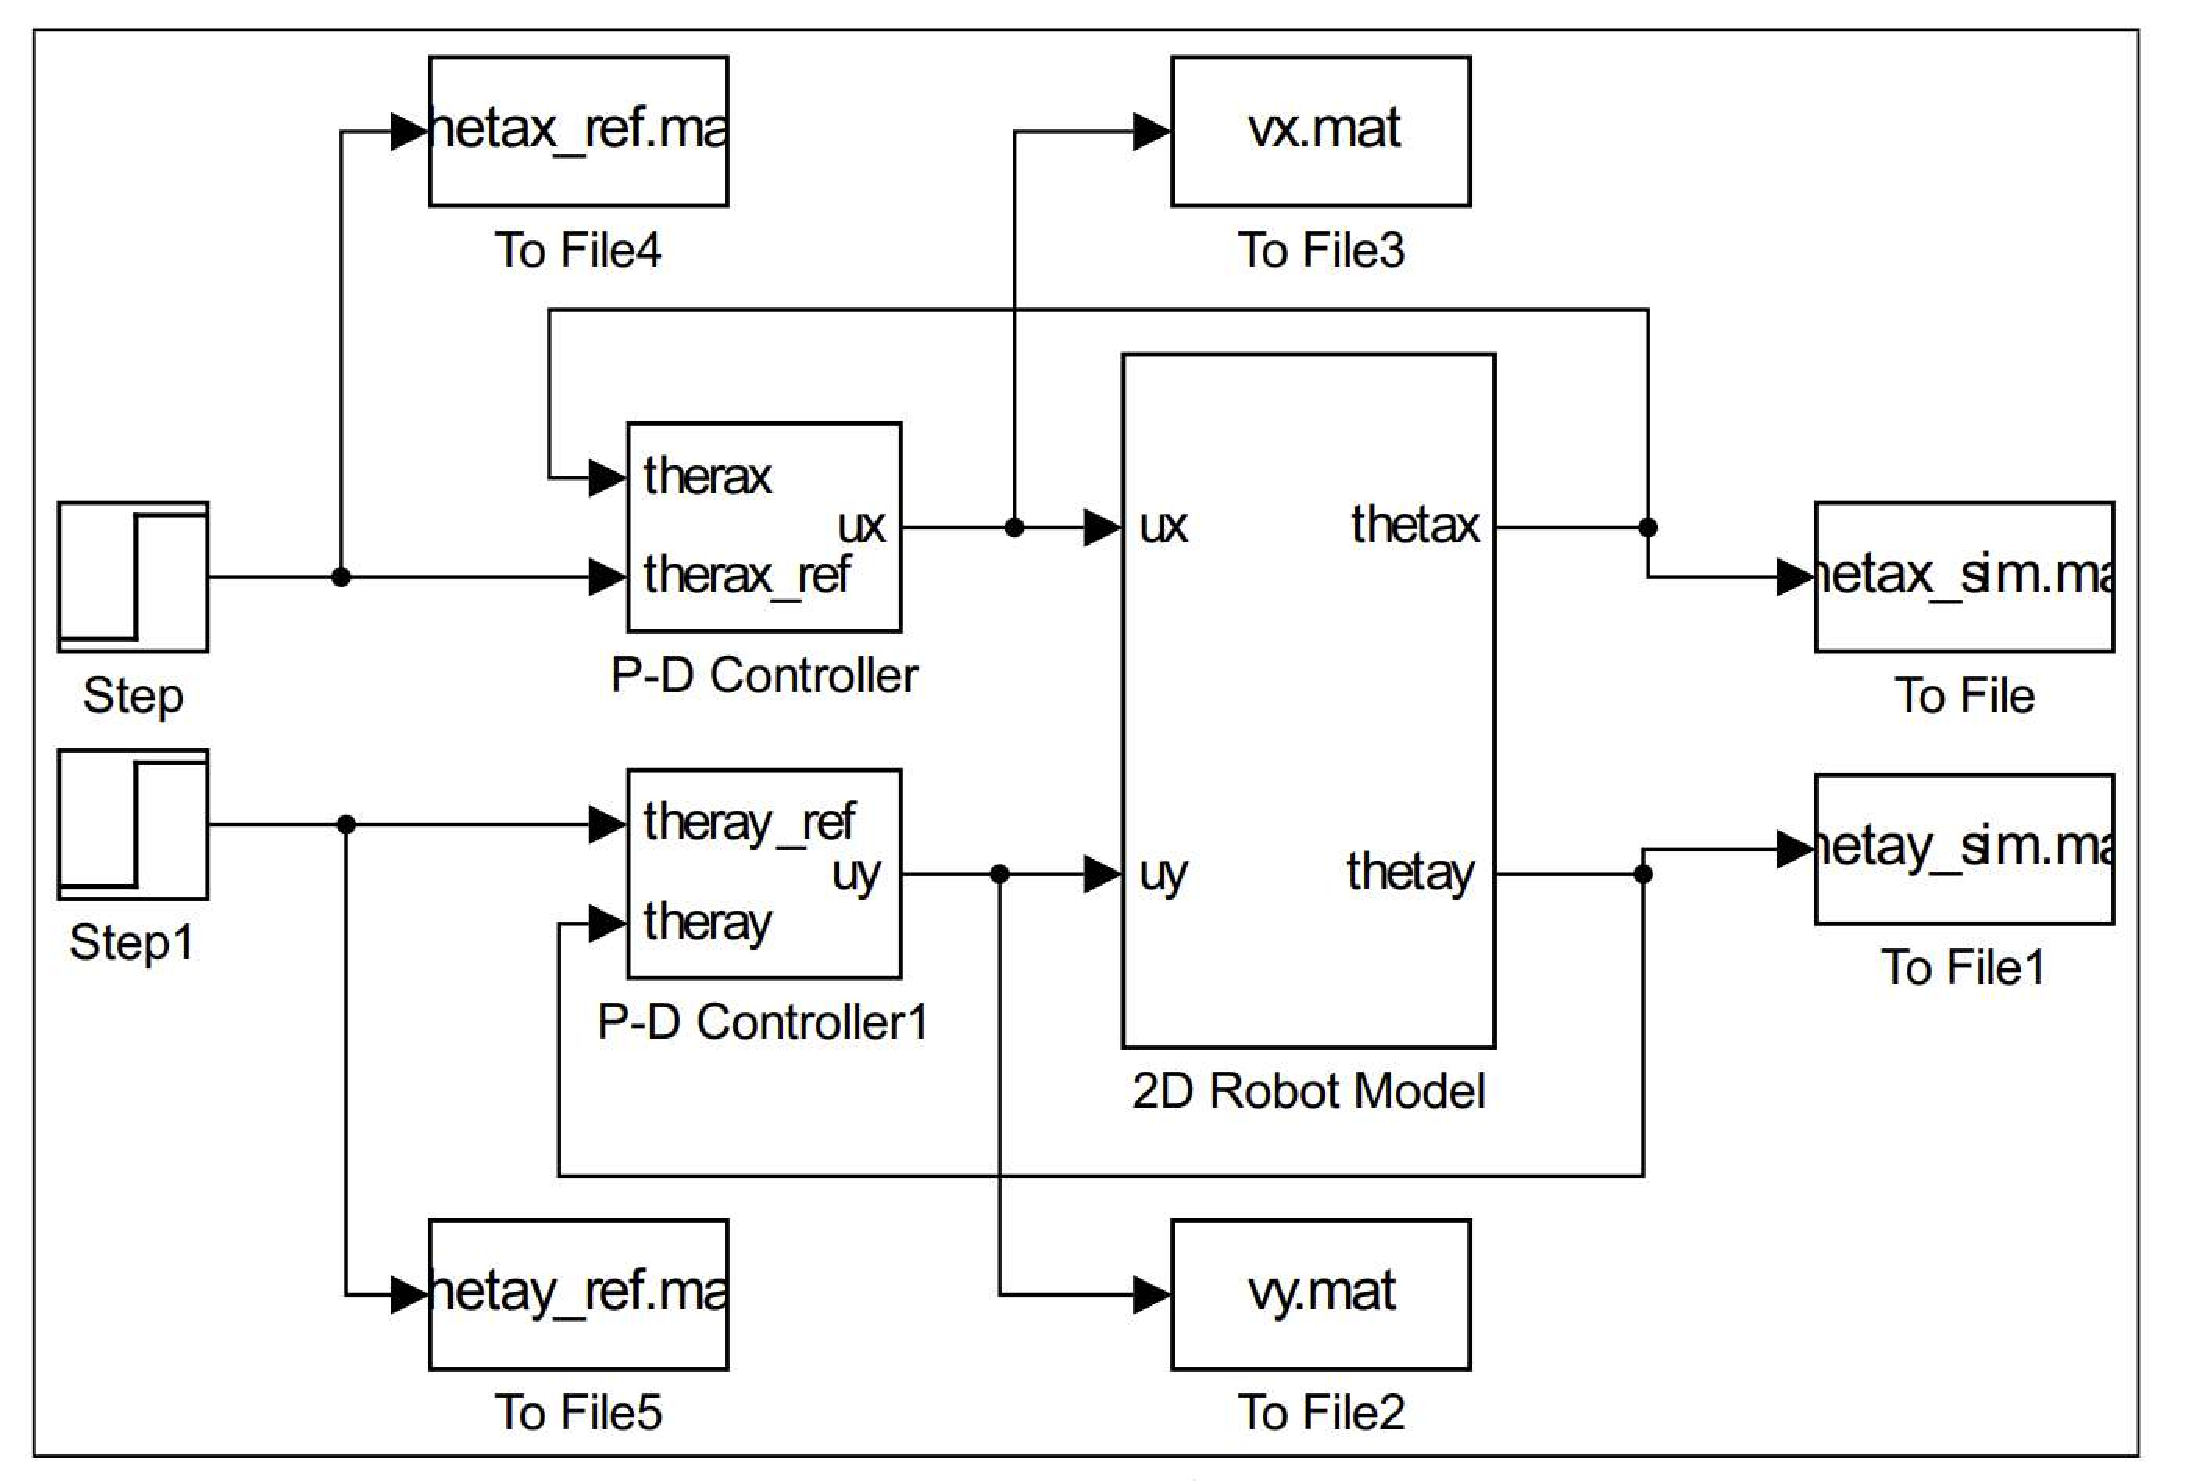
\includegraphics[width=\linewidth]{figure/sim_PD_slx.pdf}
        \caption{シミュレーションモデル ``sim\_PD.slx''}
    \end{subfigure}
    
    \vspace{0.5cm}
    
    \begin{subfigure}{0.8\linewidth}
        \centering
        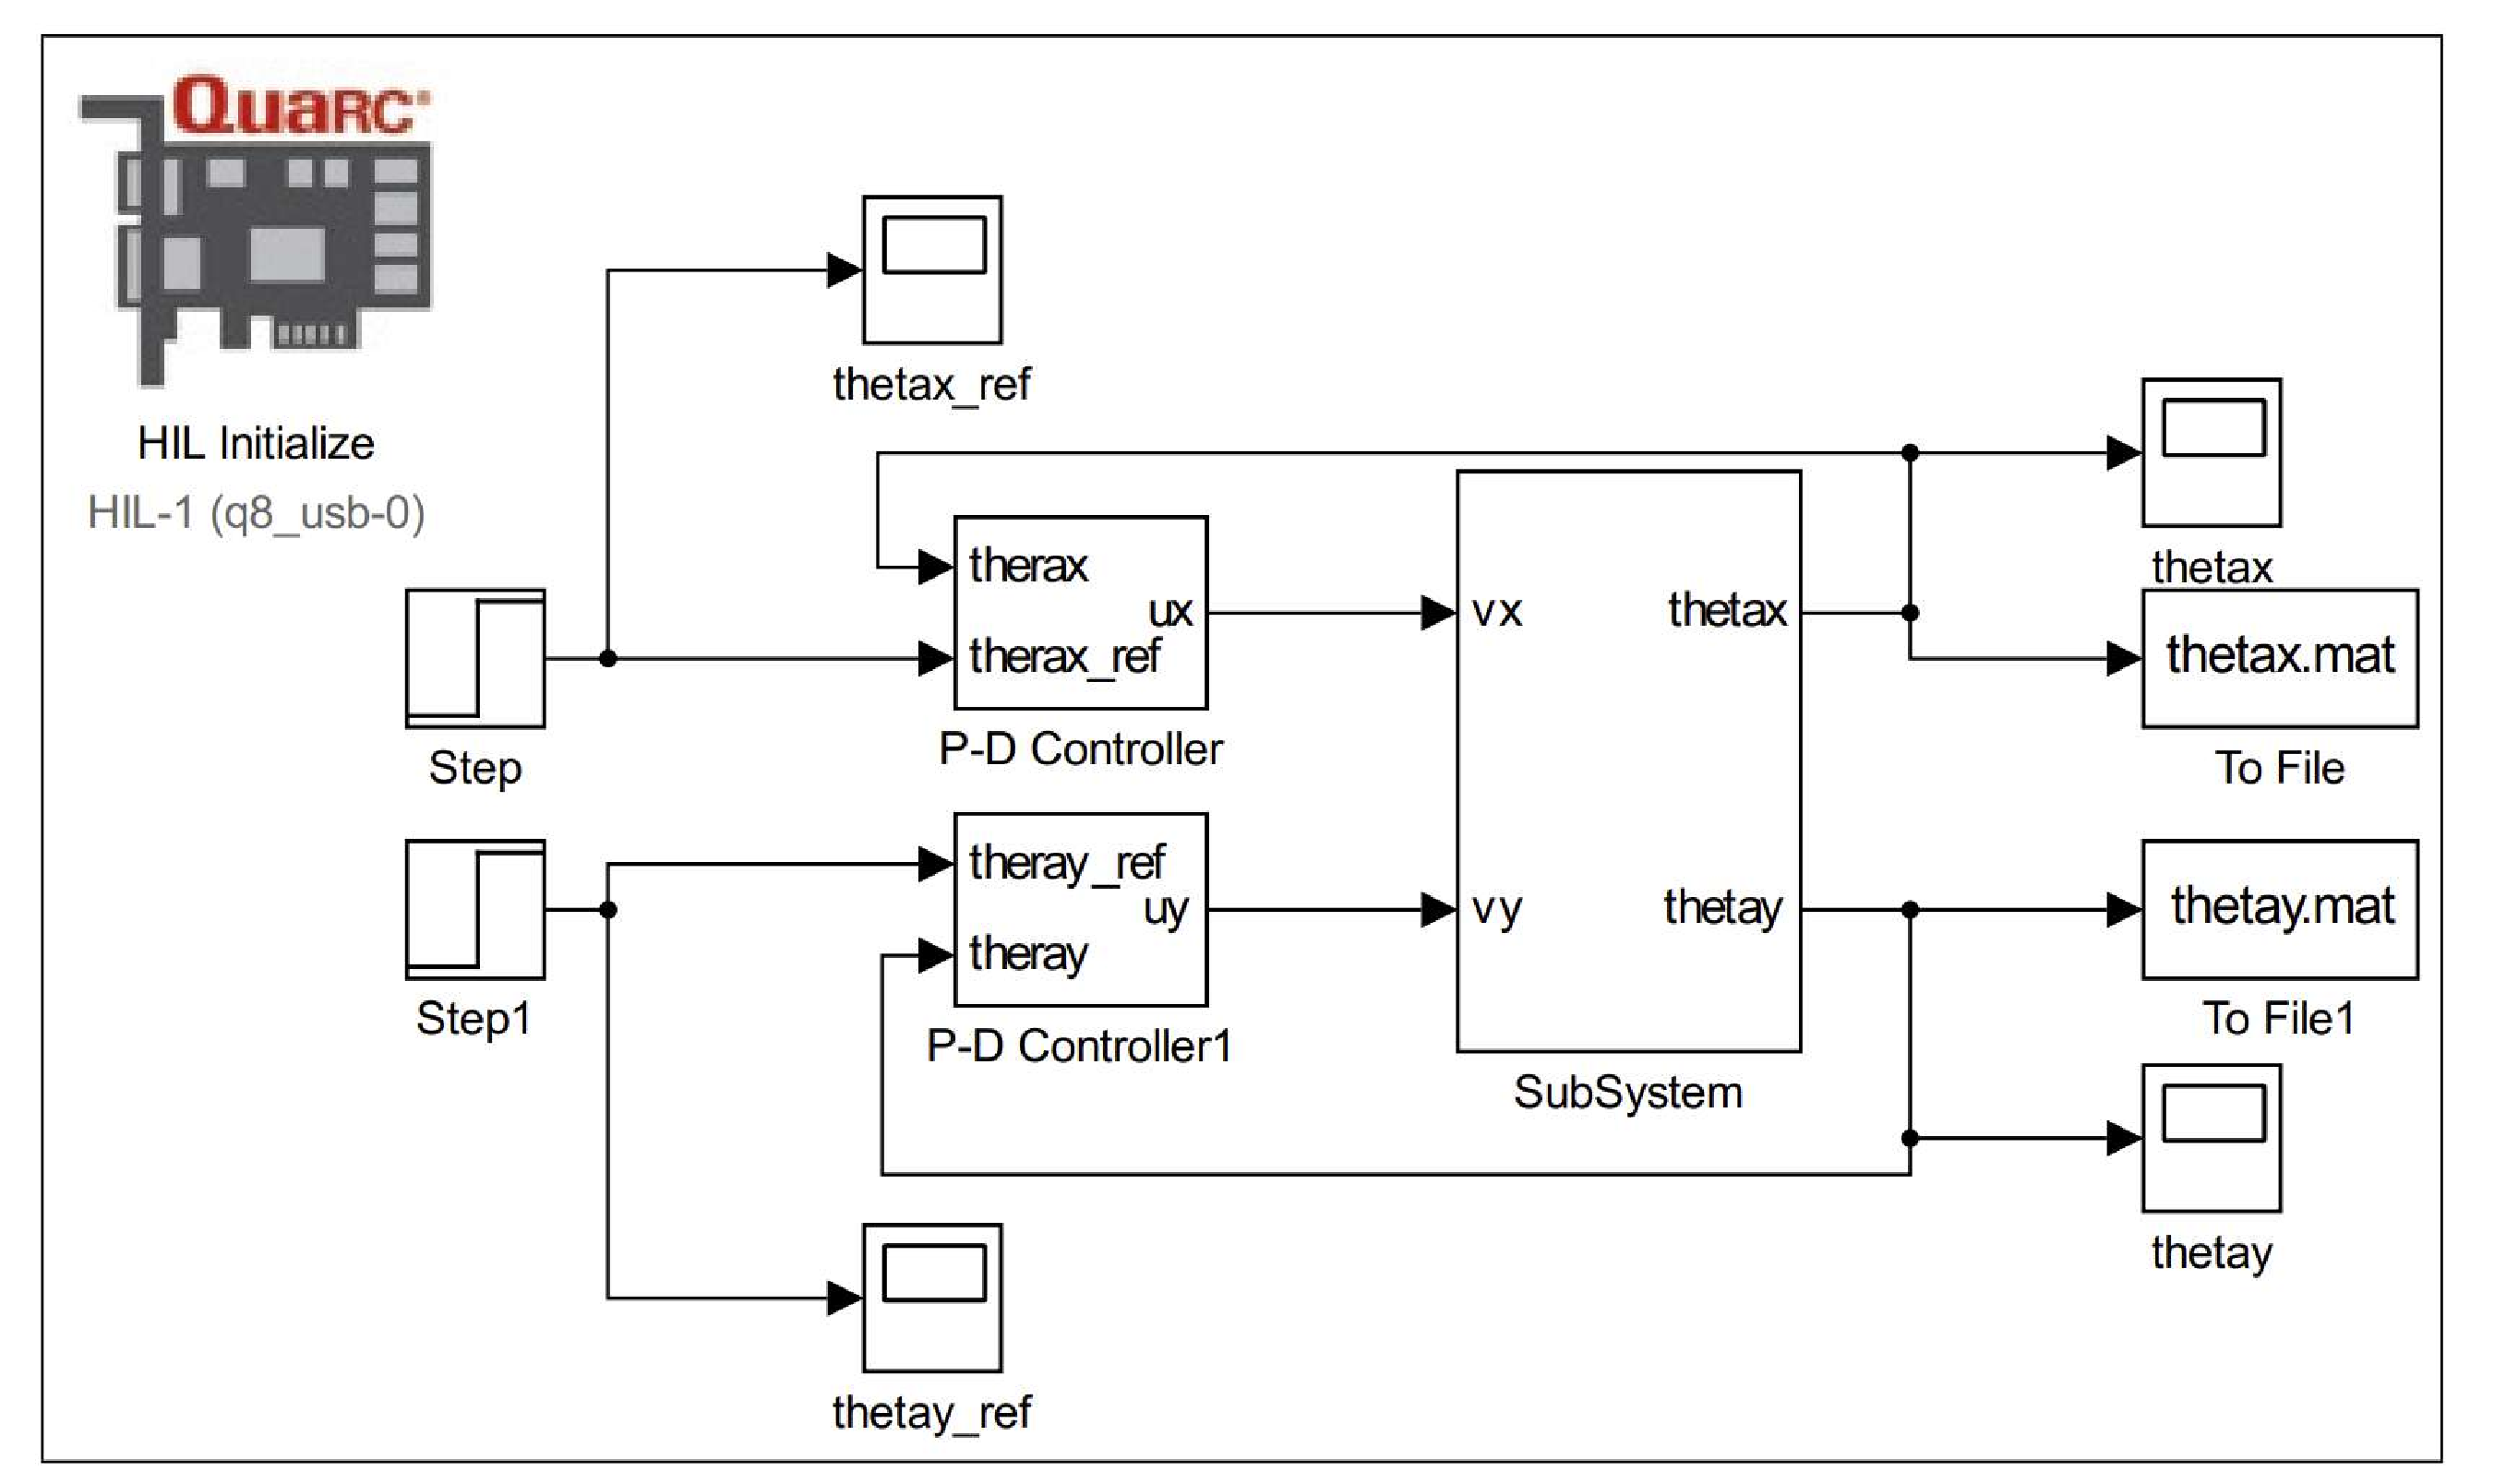
\includegraphics[width=\linewidth]{figure/ex_PD_slx.pdf}
        \caption{実機実験モデル ``ex\_PD.slx''}
    \end{subfigure}
    
    \vspace{0.5cm}
    
    \begin{subfigure}{0.8\linewidth}
        \centering
        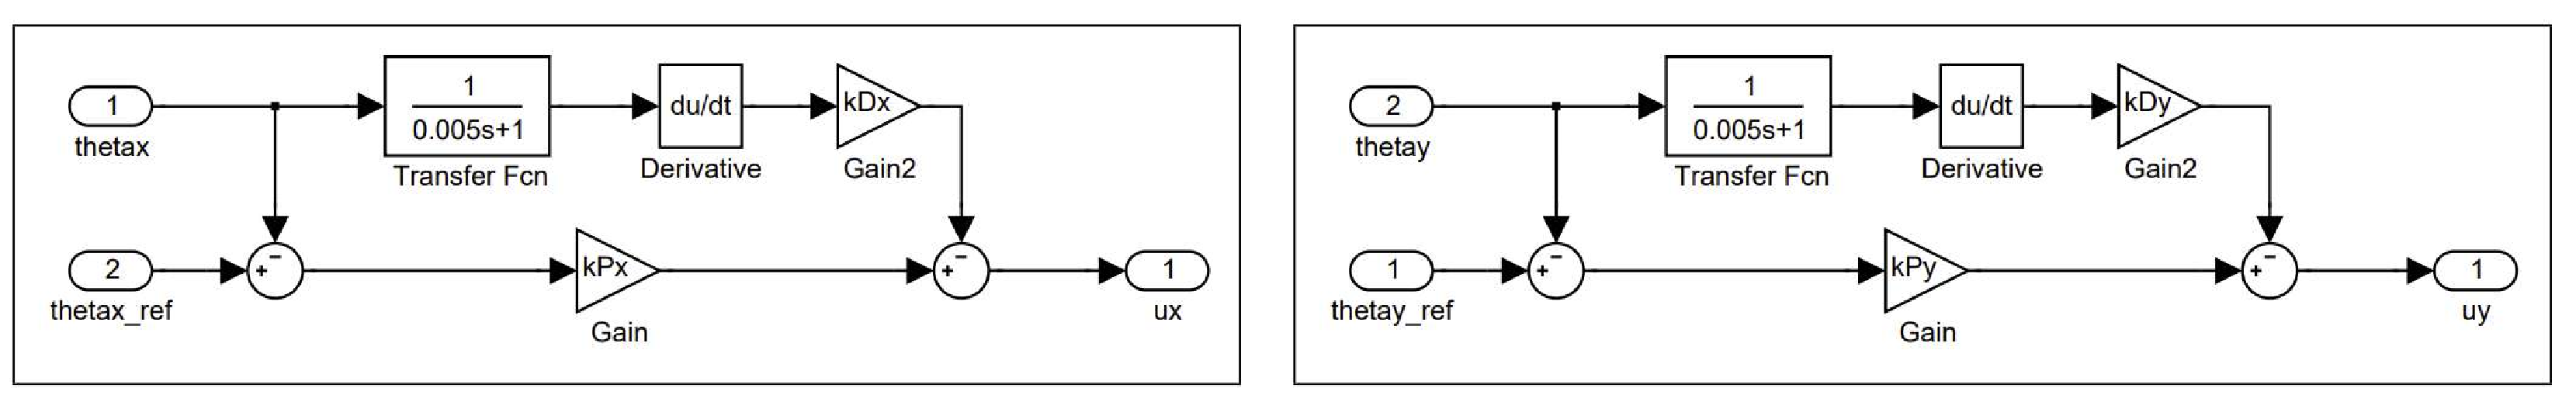
\includegraphics[width=\linewidth]{figure/PD_Controller_detail.pdf}
        \caption{Subsystem ``PD Controller'', ``PD Controller1'' の内容}
    \end{subfigure}
    
    \caption{P--D 制御の Simulink モデル}
    \label{fig:pd_simulink_model}
\end{figure}

\subsubsection{I--PD制御}
\subsubsection{パラメータ設定}

P 制御や P--D 制御はコントローラに積分器 \(1/s\) を含んでいないため,クローン摩擦の影響でステップ応答に定常偏差が生じた.そこで,コントローラに積分器 \(1/s\) を含ませることによって,ステップ状の目標値に対する定常偏差を解消することを考える.

I--PD コントローラ(比例・微分先行型 PID コントローラ)

\begin{equation}
\left\{
\begin{aligned}
v_x(t) &= -k_{Px} \theta_x(t) + k_{Ix} \int_0^t e_x(\tau) d\tau - k_{Dx} \frac{d\theta_x(t)}{dt} \\
v_y(t) &= -k_{Py} \theta_y(t) + k_{Iy} \int_0^t e_y(\tau) d\tau - k_{Dy} \frac{d\theta_y(t)}{dt}
\end{aligned}
\right.
\Longleftrightarrow
\left\{
\begin{aligned}
v_x(s) &= -k_{Px} \theta_x(s) + \frac{k_{Ix}}{s} e_x(s) - k_{Dx}s \theta_x(s) \\
v_y(s) &= -k_{Py} \theta_y(s) + \frac{k_{Iy}}{s} e_y(s) - k_{Dx}s \theta_y(s)
\end{aligned}
\right.
\tag{5.12}
\end{equation}

を用いると,\( \theta_x^{ref}(s) \) から \( \theta_x(s) \) への伝達関数は 3 次遅れ要素

\begin{equation}
\left\{
\begin{aligned}
T_x(s) &= \frac{b_x k_{Ix}}{s^3 + (a_x + b_x k_{Dx})s^2 + b_x k_{Px}s + b_x k_{Ix}} \\
T_y(s) &= \frac{b_y k_{Iy}}{s^3 + (a_y + b_y k_{Dx})s^2 + b_y k_{Py}s + b_y k_{Iy}}
\end{aligned}
\right.
\tag{5.13}
\end{equation}

となる.したがって,(5.13) 式を規範モデル

\begin{equation}
\left\{
\begin{aligned}
T_{Mx}(s) &= \frac{\omega_{Mx}^3}{s^3 + \alpha_{Mx2} \omega_{Mx}^2 s^2 + \alpha_{Mx1} \omega_{Mx}s + \omega_{Mx}^3} \\
T_{My}(s) &= \frac{\omega_{My}^3}{s^3 + \alpha_{My2} \omega_{My}^2 s^2 + \alpha_{My1} \omega_{My}s + \omega_{My}^3}
\end{aligned}
\right.
\tag{5.14}
\end{equation}

と完全に一致させるには

\begin{equation}
\left\{
\begin{aligned}
k_{Ix} &= \frac{\omega_{Mx}^3}{b_x}, \quad k_{Px} = \frac{\alpha_{Mx1} \omega_{Mx}^2}{b_x}, \quad k_{Dx} = \frac{\alpha_{Mx2} \omega_{Mx} - a_x}{b_x} \\
k_{Iy} &= \frac{\omega_{My}^3}{b_y}, \quad k_{Py} = \frac{\alpha_{My1} \omega_{My}^2}{b_y}, \quad k_{Dx} = \frac{\alpha_{My2} \omega_{My} - a_y}{b_y}
\end{aligned}
\right.
\tag{5.15}
\end{equation}

と選べばよい.ただし,\(\omega_{Mx}, \omega_{My}\) は速度応答に関するパラメータ,\(\alpha_{M1x}, \alpha_{M2x}, \alpha_{M1y}, \alpha_{M2y}\) は減衰性に関するパラメータであり,

\paragraph{規範モデルの標準形}
\begin{itemize}
    \item \textbf{パターワース標準形}:
    \[
    \left\{
    \begin{aligned}
        \alpha_{M1x} = 2, \quad \alpha_{M2x} = 2 \\
        \alpha_{M1y} = 2, \quad \alpha_{M2y} = 2
    \end{aligned}
    \right.
    \]
    
    \item \textbf{二項標準形}:
    \[
    \left\{
    \begin{aligned}
        \alpha_{M1x} = 3, \quad \alpha_{M2x} = 3 \\
        \alpha_{M1y} = 3, \quad \alpha_{M2y} = 3
    \end{aligned}
    \right.
    \]
    
    \item \textbf{ITAE 最小標準形}:
    \[
    \left\{
    \begin{aligned}
        &\alpha_{M1x} = 2.15, &\alpha_{M2x} = 1.75\\
        &\alpha_{M1y} = 2.15, &\alpha_{M2y} = 1.75
    \end{aligned}
    \right.
    \]
\end{itemize}

\noindent
が用いられることが多い.

\bigskip

\noindent
なお,実際には高周波成分の観測雑音を除去するため,次式の I--PD コントローラを用いることになる:

\begin{equation}
\left\{
\begin{aligned}
v_x(s) &= -k_{Px} \theta_x(s) + \frac{k_{Ix}}{s} e_x(s) - \frac{k_{Dx}s}{1 + T_{dx}s} \theta_x(s) \\
v_y(s) &= -k_{Py} \theta_y(s) + \frac{k_{Iy}}{s} e_y(s) - \frac{k_{Dy}s}{1 + T_{dy}s} \theta_y(s)
\end{aligned}
\right.
\tag{5.16}
\end{equation}

\subsubsection{シミュレーションと実験}
\fbox{\textbf{ステップ 1}}:
パラメータを記述した M ファイル ``armpara.m'' および (5.15) 式により I--PD コントローラのパラメータを設計する M ファイル ``armIPD.m'',シミュレーションモデル ``sim\_IPD.slx''(図 5.5 (a)),実機実験モデル ``ex\_IPD.slx''(図 5.5 (b))を作成し,C:\textbackslash robot\textbackslash IPDcont に保存する.

\fbox{\textbf{ステップ 2}}:
アームの角度を 0 にし,$\omega_{Mx} = 30$, $\alpha_{M1x} = 2$, $\alpha_{M2x} = 2$ と指定し,実験する.ただし,得られた MAT ファイル ``thetax.mat'' の名前を ``thetaxb.mat'' に変更する.

\fbox{\textbf{ステップ 3}}:
アームの角度を 0 にし,$\omega_{Mx} = 30$, $\alpha_{M1x} = 3$, $\alpha_{M2x} = 3$ と指定し,実験する.ただし,得られた MAT ファイル ``thetax.mat'' の名前を ``thetax2.mat'' に変更する.

\fbox{\textbf{ステップ 4}}:
アームの角度を 0 にし,$\omega_{Mx} = 30$, $\alpha_{M1x} = 2.15$, $\alpha_{M2x} = 1.75$ と指定し,実験する.ただし,得られた MAT ファイル ``thetax.mat'' の名前を ``thetaxi.mat'' に変更する.

\begin{figure}[H]
    \centering
    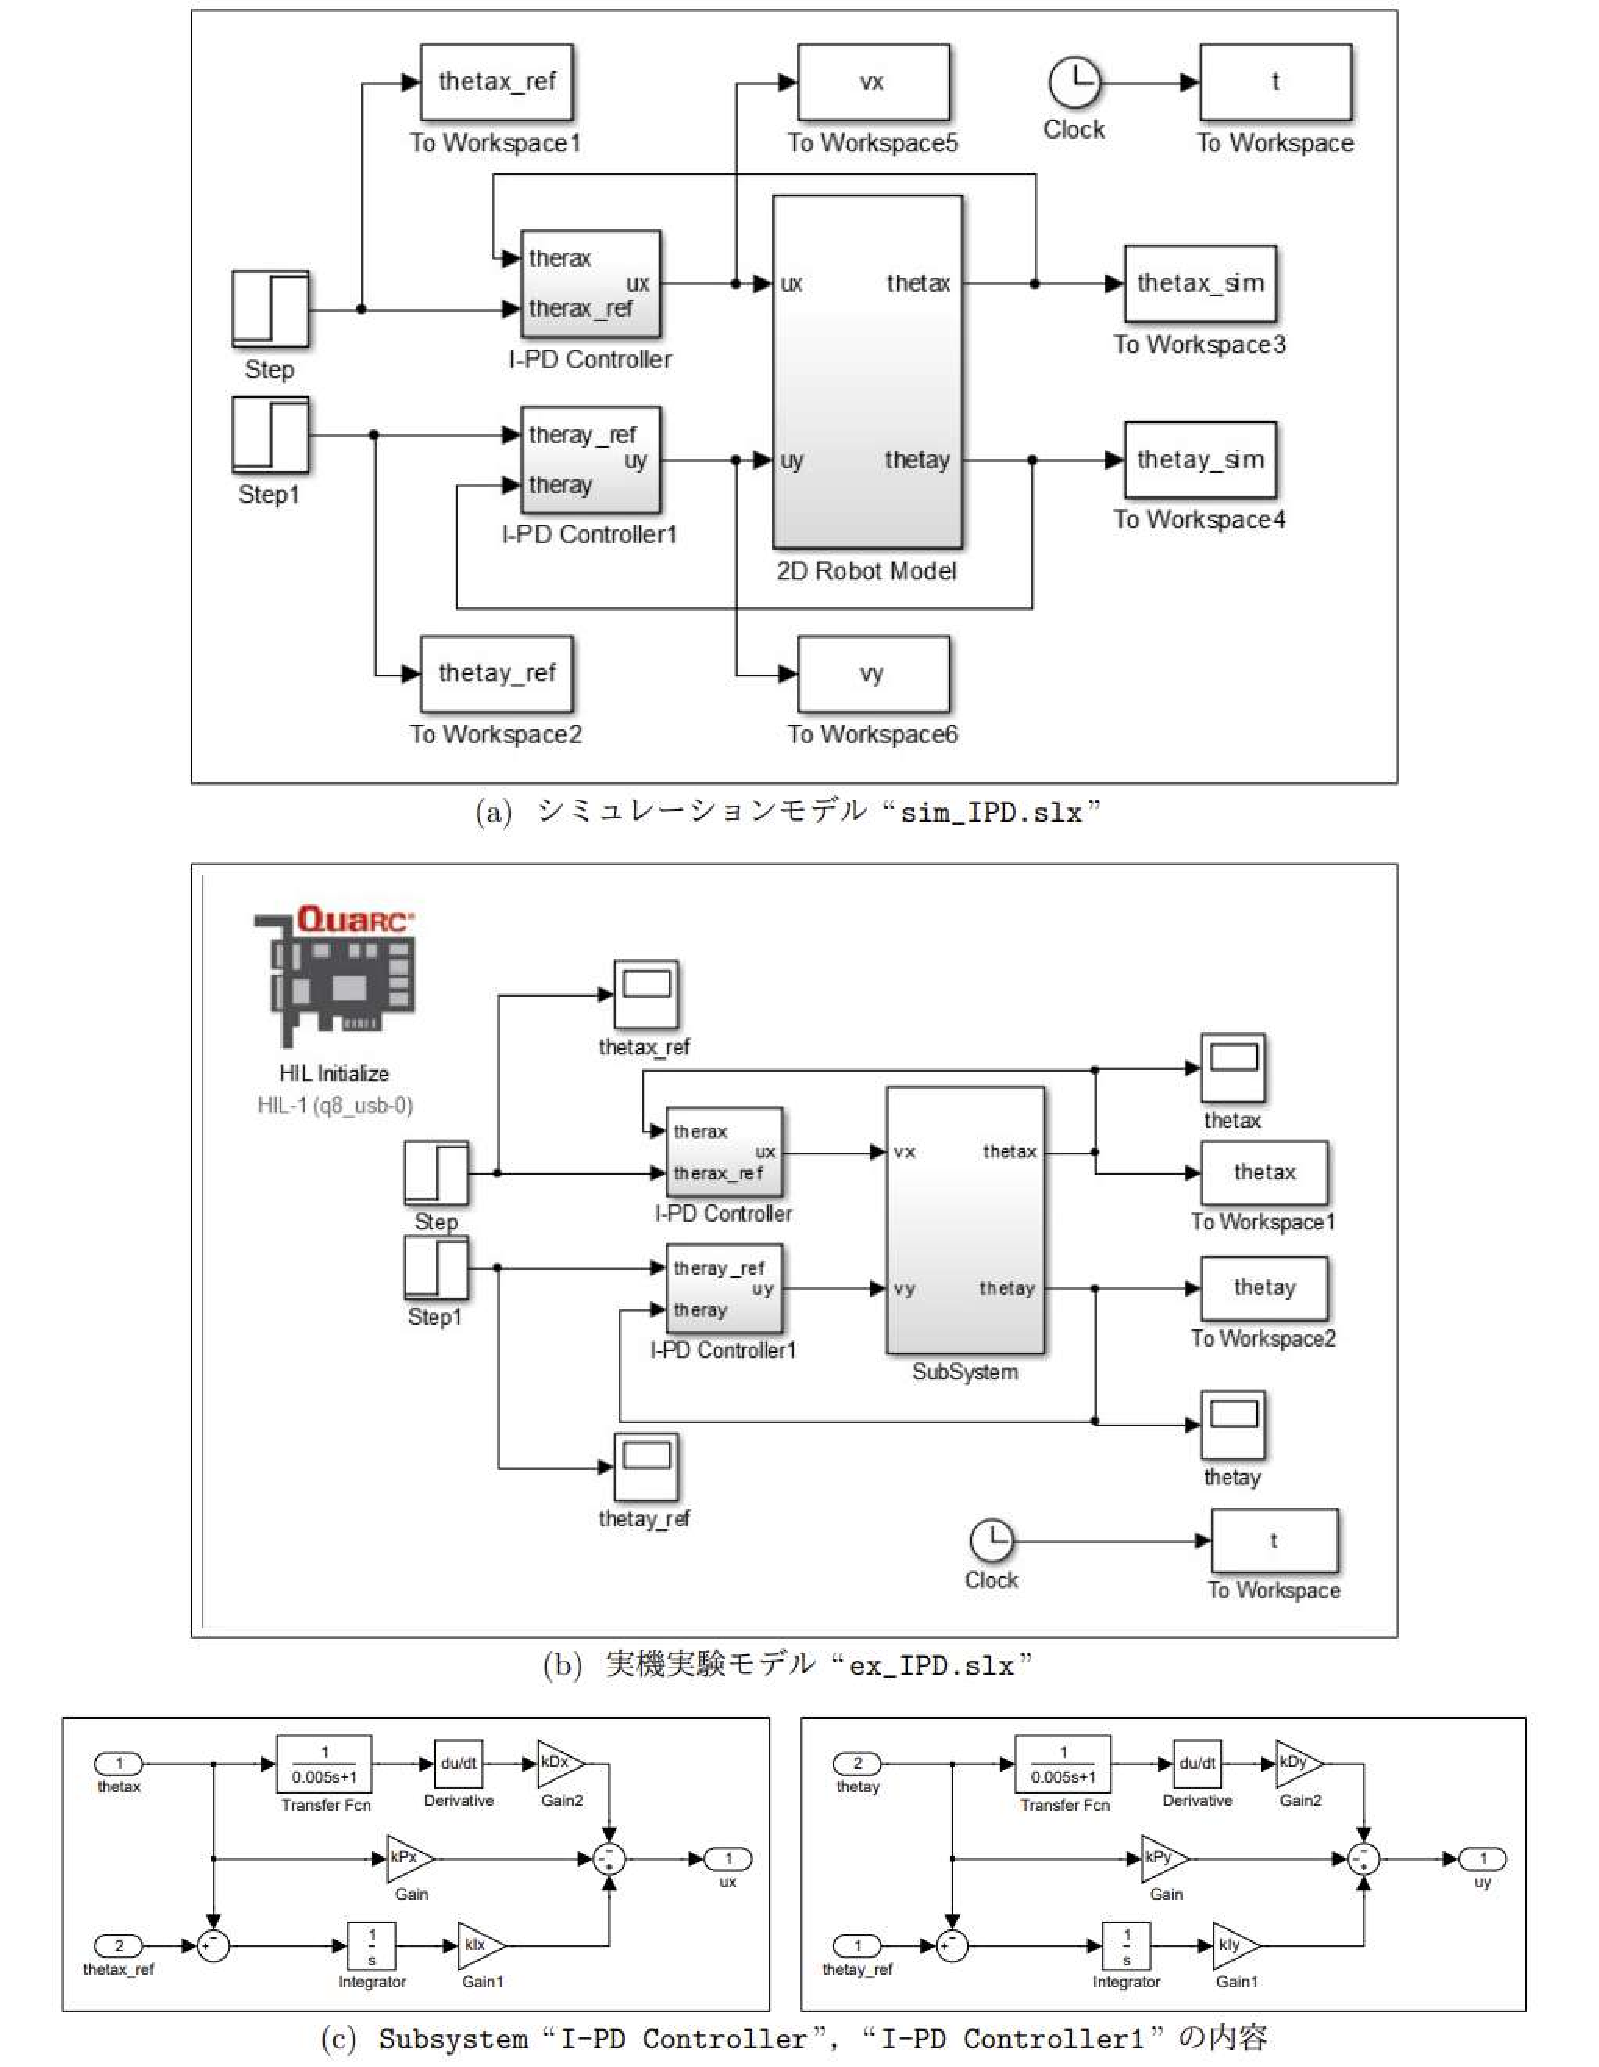
\includegraphics[width=0.95\linewidth]{figure/ipd_simulink_model.pdf}
    \caption{I--PD 制御の Simulink モデル}
    \label{fig:ipd_simulink}
\end{figure}

\subsection{実験結果}
\begin{figure}[H]
    \centering
    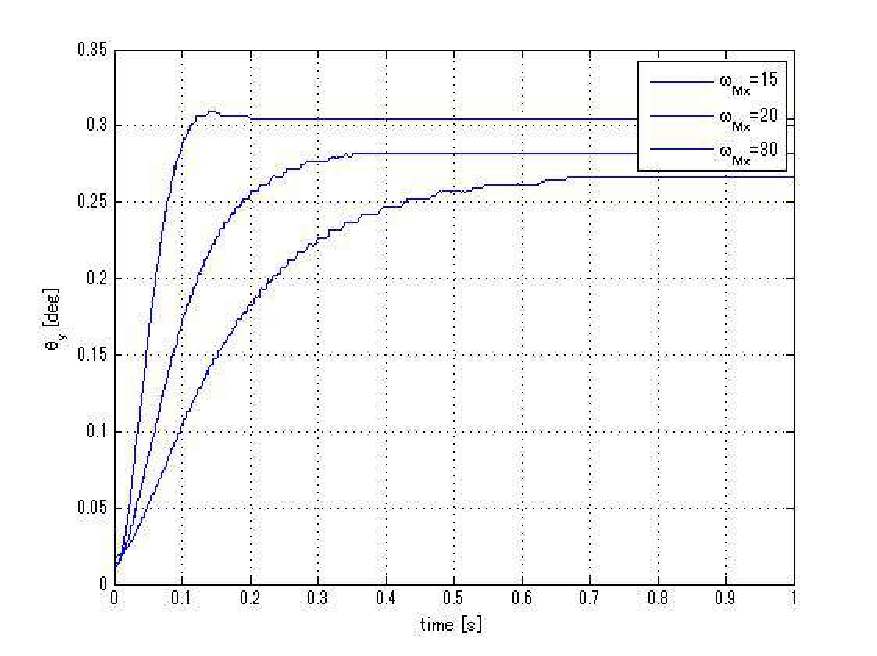
\includegraphics[width=0.6\linewidth]{figure/plot_figure.pdf}
    \caption{P制御の応答}
    \label{fig:step_response}
\end{figure}

図~\ref{fig:step_response} に示すように,P制御では速応性が改善される一方でオーバーシュートが大きくなることが確認された.

\begin{figure}[H]
    \centering
    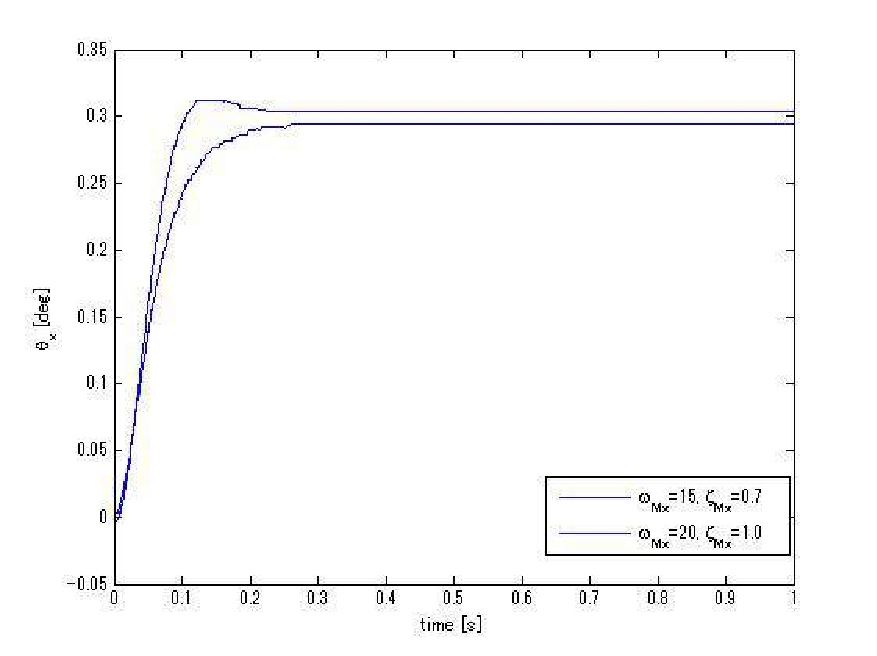
\includegraphics[width=0.6\linewidth]{figure/ex_pd_hidari.pdf}
    \caption{P--D制御の応答}
    \label{fig:pd_response}
\end{figure}

また,図~\ref{fig:pd_response} に示すように,P--D制御では安定度が改善され,たが定常偏差が残るようになった.

\begin{figure}[H]
    \centering
    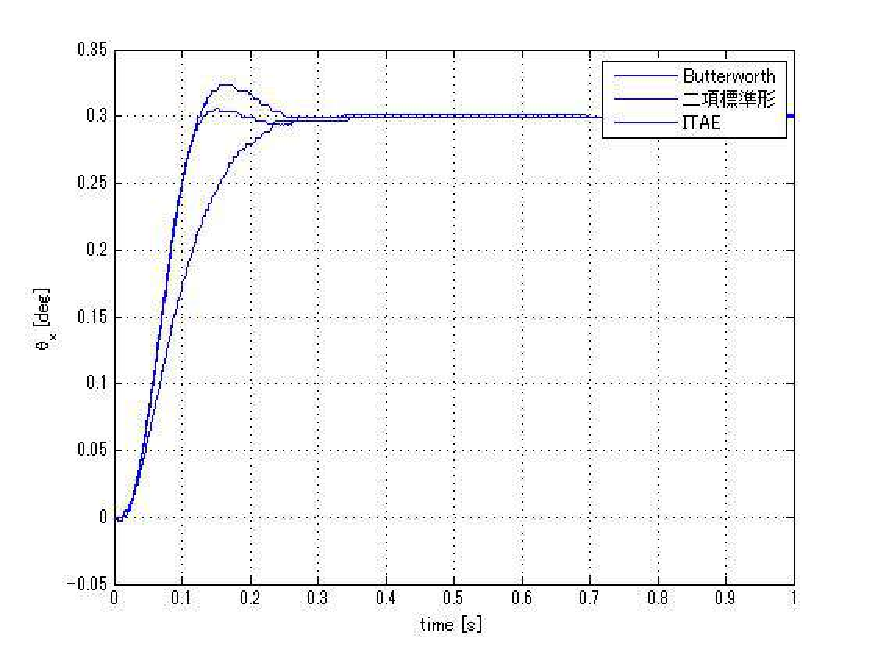
\includegraphics[width=0.6\linewidth]{figure/ex_ipd.pdf}
    \caption{I--PD制御の応答}
    \label{fig:ipd_result}
\end{figure}

図~\ref{fig:ipd_result} に示すように,I--PD制御では定常偏差が解消された.
\subsection{考察}
P制御では速応性が向上するが,オーバーシュートが大きくなるため,減衰係数の調整が必要である.P--D制御では安定度が向上し,振動が抑制された.
さらに,I--PD制御では定常偏差が解消され,目標値への追従性が向上した.
